
\section{Calculations \& Graphs}

\vspace{-0.5cm}
\singlespacing

%------- Force --------%

\subsection{Force \& Acceleration} 

{\centering
\begin{equation}
	F = ma 
	\label{eq:NetForce}
\end{equation}
\begin{equation}
	a = \frac{F}{m} 
	\label{eq:CalcAcc}
\end{equation}
\begin{align*}
	\boldsymbol{F} &: \text{Force of object} \\
	\boldsymbol{m} &: \text{mass of object} \\
	\boldsymbol{a} &: \text{acceleration of object}
\end{align*}}

\subsubsection{Sample Calculation \\ {\normalfont \small\textit{Force of hanging mass at 10\,grams}}}

{\centering
\text{\textbf{Knowns:}}
\begin{align*}
	m &= \boldsymbol{.01\,\text{\textbf{kg}}} \\
	a &= \boldsymbol{9.8\,\text{\textbf{m/s}}^2}
\end{align*}

\text{\textbf{Calculating Force of Hanging Mass:}}
\begin{align*}
	F &= ma \\
	&= (.01)(9.8) \\
	F &= \boxed{0.098\,\text{N}}
\end{align*}}

\subsubsection{Sample Calculation \\ {\normalfont \small\textit{Acceleration of glider when hanging mass at 10 grams}}}

{\centering
\text{\textbf{Knowns:}}
\begin{align*}
	F &= \boldsymbol{0.098\,\text{\textbf{N}}} \\
	m &= \boldsymbol{0.3409\,\text{\textbf{kg}}}
\end{align*}

\text{\textbf{Calculating Expected Acceleration of Glider:}}
\begin{align*}
	a &= \frac{F}{m} \\
	&= \frac{0.098}{0.3409} \\
	a &= \boxed{0.2874\,\text{m/s}^2}
\end{align*}}


\newpage
%------- ACCELERATION BETWEEN TWO POINTS WITH INITIAL VELOCITY CLOSE TO ZERO--------%

\subsection{Acceleration Between Two Points with Initial Velocity Close to Zero} 

{\centering
\begin{equation}
	a = \frac{2\Delta{x}}{t^2} 
	\label{eq:MeasuredAcc}
\end{equation}
\begin{align*}
	\boldsymbol{\Delta{x}} &: \text{Distance between photogates} \\
\boldsymbol{t} &: \text{average time between photogates}
\end{align*}}

\subsubsection{Sample Calculation \\ {\normalfont \small\textit{Measured acceleration of glider with hanging mass at 10 grams}}}

{\centering
\textbf{Knowns:}
\begin{align*}
	\Delta{x} &= \boldsymbol{0.669\,\text{\textbf{m}}} \\
	t &= \boldsymbol{2.058\,\text{\textbf{s}}}
\end{align*}

\textbf{Calculating Measured Acceleration of Glider:}
\begin{align*}
	a &= \frac{2\Delta{x}}{t^2} \\
	&= \frac{(2)(0.669)}{(2.058)^2} \\
	a &= \boxed{0.3156\,\text{m/s}^2}
\end{align*}}

%------- ACCELERATION BETWEEN TWO POINTS --------%

%------- AVERAGE VALUE --------%
\subsection{Average Value Formula} 

\begin{align*}
	\overline{a} = \frac{\text{sum of values}}{\text{total \# of values}} 
\end{align*}

\subsubsection{Sample Calculation \\ {\normalfont \small\textit{average time between photogates of glider with hanging mass at 10 grams }}}


\begin{align*}
	\overline{a}&=\frac{\text{sum of values}}{\text{total \# of values}} \\ \\
							&= \frac{2.043+2.067+2.067}{3} \\ \\
	\overline{a}&= \boxed{2.059\,\text{s}}
\end{align*}
%------- AVERAGE VALUE --------%

%------- STANDARD DEVIATION --------%
\subsection{Standard Deviation Formula}

\begin{align*}
		\sigma &= \sqrt{\frac{\Sigma(x_i -\overline{a})^2}{N}} \\
		 &= \sqrt{\frac{SS}{N}} \\ \\
		\textbf{N} &:\, \text{Total number of values} \\
		\overline{\textbf{a}} &:\, \text{Average value} \\
		\textbf{x\textsubscript{i}} &:\, \text{Each value from the data set} \\
		\textbf{SS} &:\, \text{Sum of squares} 
\end{align*}

\subsubsection{Sample Calculation \\ {\normalfont \small\textit{std of photogate times with hanging mass at 10 grams }}}

\begin{align*}
	\sigma &= \sqrt{\frac{(2.043-\overline{a})^2 + ... + (2.067-\overline{a})^2}{3}} \\
		 &= \sqrt{\frac{0.000384}{3}} \\
		 &= \boxed{0.01131\, \text{s}}
\end{align*}
%------- STANDARD DEVIATION --------%

%------- RELATIVE ERROR --------%
\subsection{Relative Error Formula}

\begin{align*}
	RE &= \left| {\frac{V_A-V_E}{V_E}} \right|\: \text{x}\: 100\% \\ \\
	\boldsymbol{V_A} &:\, \text{Actual value observed} \\
	\boldsymbol{V_E} &:\, \text{Expected value} 
\end{align*}

\subsubsection{Sample Calculation \\ {\normalfont \small\textit{acceleration of glider on air track with hanging mass at 10 grams - measured vs calculations}}}

\begin{align*}
	RE &= \left| {\frac{V_A-V_E}{V_E}} \right|\: \text{x}\: 100\% \\
	 &= \left| {\frac{0.3156-0.2874}{0.2874}} \right|\: \text{x}\: 100\% \\
			RE &= \boxed{9.80\%} 
\end{align*}
%------- RELATIVE ERROR --------%

%----TABLES-----%

\begin{landscape}

\subsection{Tables}

\begin{table}[H]
\captionsetup{font=Large}
\caption{Known values}
\centering
\begin{threeparttable}
\resizebox{12cm}{!}{%
\begin{tabular}{ccccc} \toprule
	\textbf{g (m/s\textsuperscript{2})} & \textbf{x\textsubscript{1} (m)\tnote{!}} & \textbf{x\textsubscript{2} (m)\tnote{!}} & \textbf{$\Delta$x (m)} & \textbf{M (kg)\tnote{!!}}  \\ \toprule
9.8                                 & 1.169                           & 0.5                             & 0.669                  & 0.3409           \\ \bottomrule
\end{tabular}
}
\begin{tablenotes}\normalsize
	\item[!] Positions of photogates 1 and 2
	\item[!!] Mass of entire system
\end{tablenotes}
\end{threeparttable}
\label{tab:knownsTab}
\end{table}
\vspace{-0.5cm}

\begin{table}[H]
\captionsetup{font=Large}
\caption{Accelerating System of Mass M - New Measurements}
\centering
\begin{threeparttable}
\resizebox{22cm}{!}{%
\begin{tabular}{ccccccccc} \toprule
\textbf{Measurement \#}                        & \textbf{1}    & \textbf{2}    & \textbf{3}    & \textbf{4}    & \textbf{5}    & \textbf{6}    & \textbf{7}     & \textbf{8}     \\ \toprule
\textbf{m (g)\tnote{!}}                        & 0.01          & 0.015         & 0.02          & 0.025         & 0.03          & 0.035         & 0.04           & 0.045          \\
\textbf{F\textsubscript{net} (N)}              & 0.098         & 0.147         & 0.196         & 0.245         & 0.294         & 0.343         & 0.392          & 0.441          \\
\textbf{a(predicted) (m/s\textsuperscript{2})} & 0.2874        & 0.4312        & 0.5749        & 0.7186        & 0.8623        & 1.0060        & 1.1498         & 1.2935         \\
\textbf{T\textsubscript{1} (s)}                & 2.043         & 1.698         & 1.515         & 1.298         & 1.223         & 1.083         & 0.9914         & 0.9405         \\
\textbf{T\textsubscript{2} (s)}                & 2.067         & 1.732         & 1.435         & 1.316         & 1.223         & 1.075         & 1.045          & 0.9811         \\
\textbf{T\textsubscript{3} (s)}                & 2.067         & 1.739         & 1.491         & 1.298         & 1.207         & 1.143         & 1.037          & 1.008          \\
\textbf{T\textsubscript{avg} (s)}              & 2.059         & 1.723         & 1.48          & 1.304         & 1.217         & 1.1           & 1.024          & 0.9765         \\
\textbf{T\textsubscript{std} (s)}              & 0.01131       & 0.0179        & 0.03351       & 0.008485      & 0.007542      & 0.03034       & 0.0236         & 0.02774        \\
\textbf{a(measured) (m/s\textsuperscript{2})}  & 0.3156        & 0.4506        & 0.6108        & 0.7868        & 0.9033        & 1.105         & 1.276          & 1.403          \\ \toprule
\textbf{Percent Error (\%)}                    & \textbf{9.80} & \textbf{4.51} & \textbf{6.25} & \textbf{9.49} & \textbf{4.75} & \textbf{9.84} & \textbf{10.98} & \textbf{8.47}  \\ \bottomrule
\end{tabular}%
}
\begin{tablenotes}\normalsize
	\item[!] Hanging mass only 
\end{tablenotes}
\end{threeparttable}
\label{tab:dataTabNew}
\end{table}

\begin{table}[H]
\centering
\captionsetup{font=Large}
\caption{Accelerating System of Mass M - Old Measurements}
\begin{threeparttable}
\resizebox{\linewidth}{!}{%
\begin{tabular}{ccccccccc} \toprule
\textbf{Measurement \#}                                                          & 1       & 2        & 3       & 4       & 5       & 6       & 7       & 8        \\ \toprule
\textbf{m (g)\tnote{!}}                        & 0.01          & 0.015         & 0.02          & 0.025         & 0.03          & 0.035         & 0.04           & 0.045          \\
\textbf{F\textsubscript{net} (N)}              & 0.098         & 0.147         & 0.196         & 0.245         & 0.294         & 0.343         & 0.392          & 0.441          \\
\textbf{a(predicted) (m/s\textsuperscript{2})} & 0.2874        & 0.4312        & 0.5749        & 0.7186        & 0.8623        & 1.0060        & 1.1498         & 1.2935         \\
$\mathbf{T_1}\textbf{ (s)}$                                                      & 2.627   & 1.970    & 1.774   & 1.664   & 1.599   & 1.463   & 1.265   & 1.172    \\
$\mathbf{T_2}\textbf{ (s)}$                                                      & 2.501   & 1.990    & 1.704   & 1.562   & 1.580   & 1.436   & 1.355   & 1.248    \\
$\mathbf{T_3}\textbf{ (s)}$                                                      & 2.630   & 1.980    & 1.727   & 1.699   & 1.538   & 1.336   & 1.298   & 1.152    \\
\begin{tabular}[c]{@{}c@{}}$\mathbf{T_\textbf{avg}}\textbf{ (s)}$\\\end{tabular} & 2.586   & 1.980    & 1.735   & 1.642   & 1.573   & 1.412   & 1.306   & 1.191    \\
\begin{tabular}[c]{@{}c@{}}$\mathbf{T_\textbf{std}}\textbf{ (s)}$\\\end{tabular} & 0.06016 & 0.008124 & 0.02923 & 0.05805 & 0.02562 & 0.05441 & 0.03683 & 0.04161  \\
\textbf{a(measured) (m/s\textsuperscript{2})}                                  & 0.2000  & 0.3411   & 0.4442  & 0.4961  & 0.5408  & 0.6710  & 0.7838  & 0.9429   \\ \toprule
\textbf{Percent Error (\%)}                                                    & \textbf{30.42} & \textbf{20.89}  & \textbf{22.73} & \textbf{30.96} & \textbf{37.29} & \textbf{33.30} & \textbf{31.83} & \textbf{27.10}  \\ \bottomrule
\end{tabular}%
}
\begin{tablenotes}\normalsize
	\item[!] Hanging mass only 
\end{tablenotes}
\end{threeparttable}
\label{tab:dataTabOld}
\end{table}

\begin{table}[H]
\centering
\captionsetup{font=Large}
\caption{Measured Acceleration - Fractional Discrepancy of Slope (Mass)}
\label{tab:slopeTab}
\resizebox{15cm}{!}      \\
\textbf{Measured (Old)} & 0.4936                                    & \multicolumn{1}{r}{36.59\%}      \\ \bottomrule
\end{tabular}
}
\end{table}
\end{landscape}
 
%----TABLES-----%

%----GRAPHS-----%

\begin{landscape}
\subsection{Graphs}
\begin{figure}[H]
	\begin{center}
		\captionsetup{font=Large}
		\caption{Force vs. Acceleration}\label{fig:GFvA}
		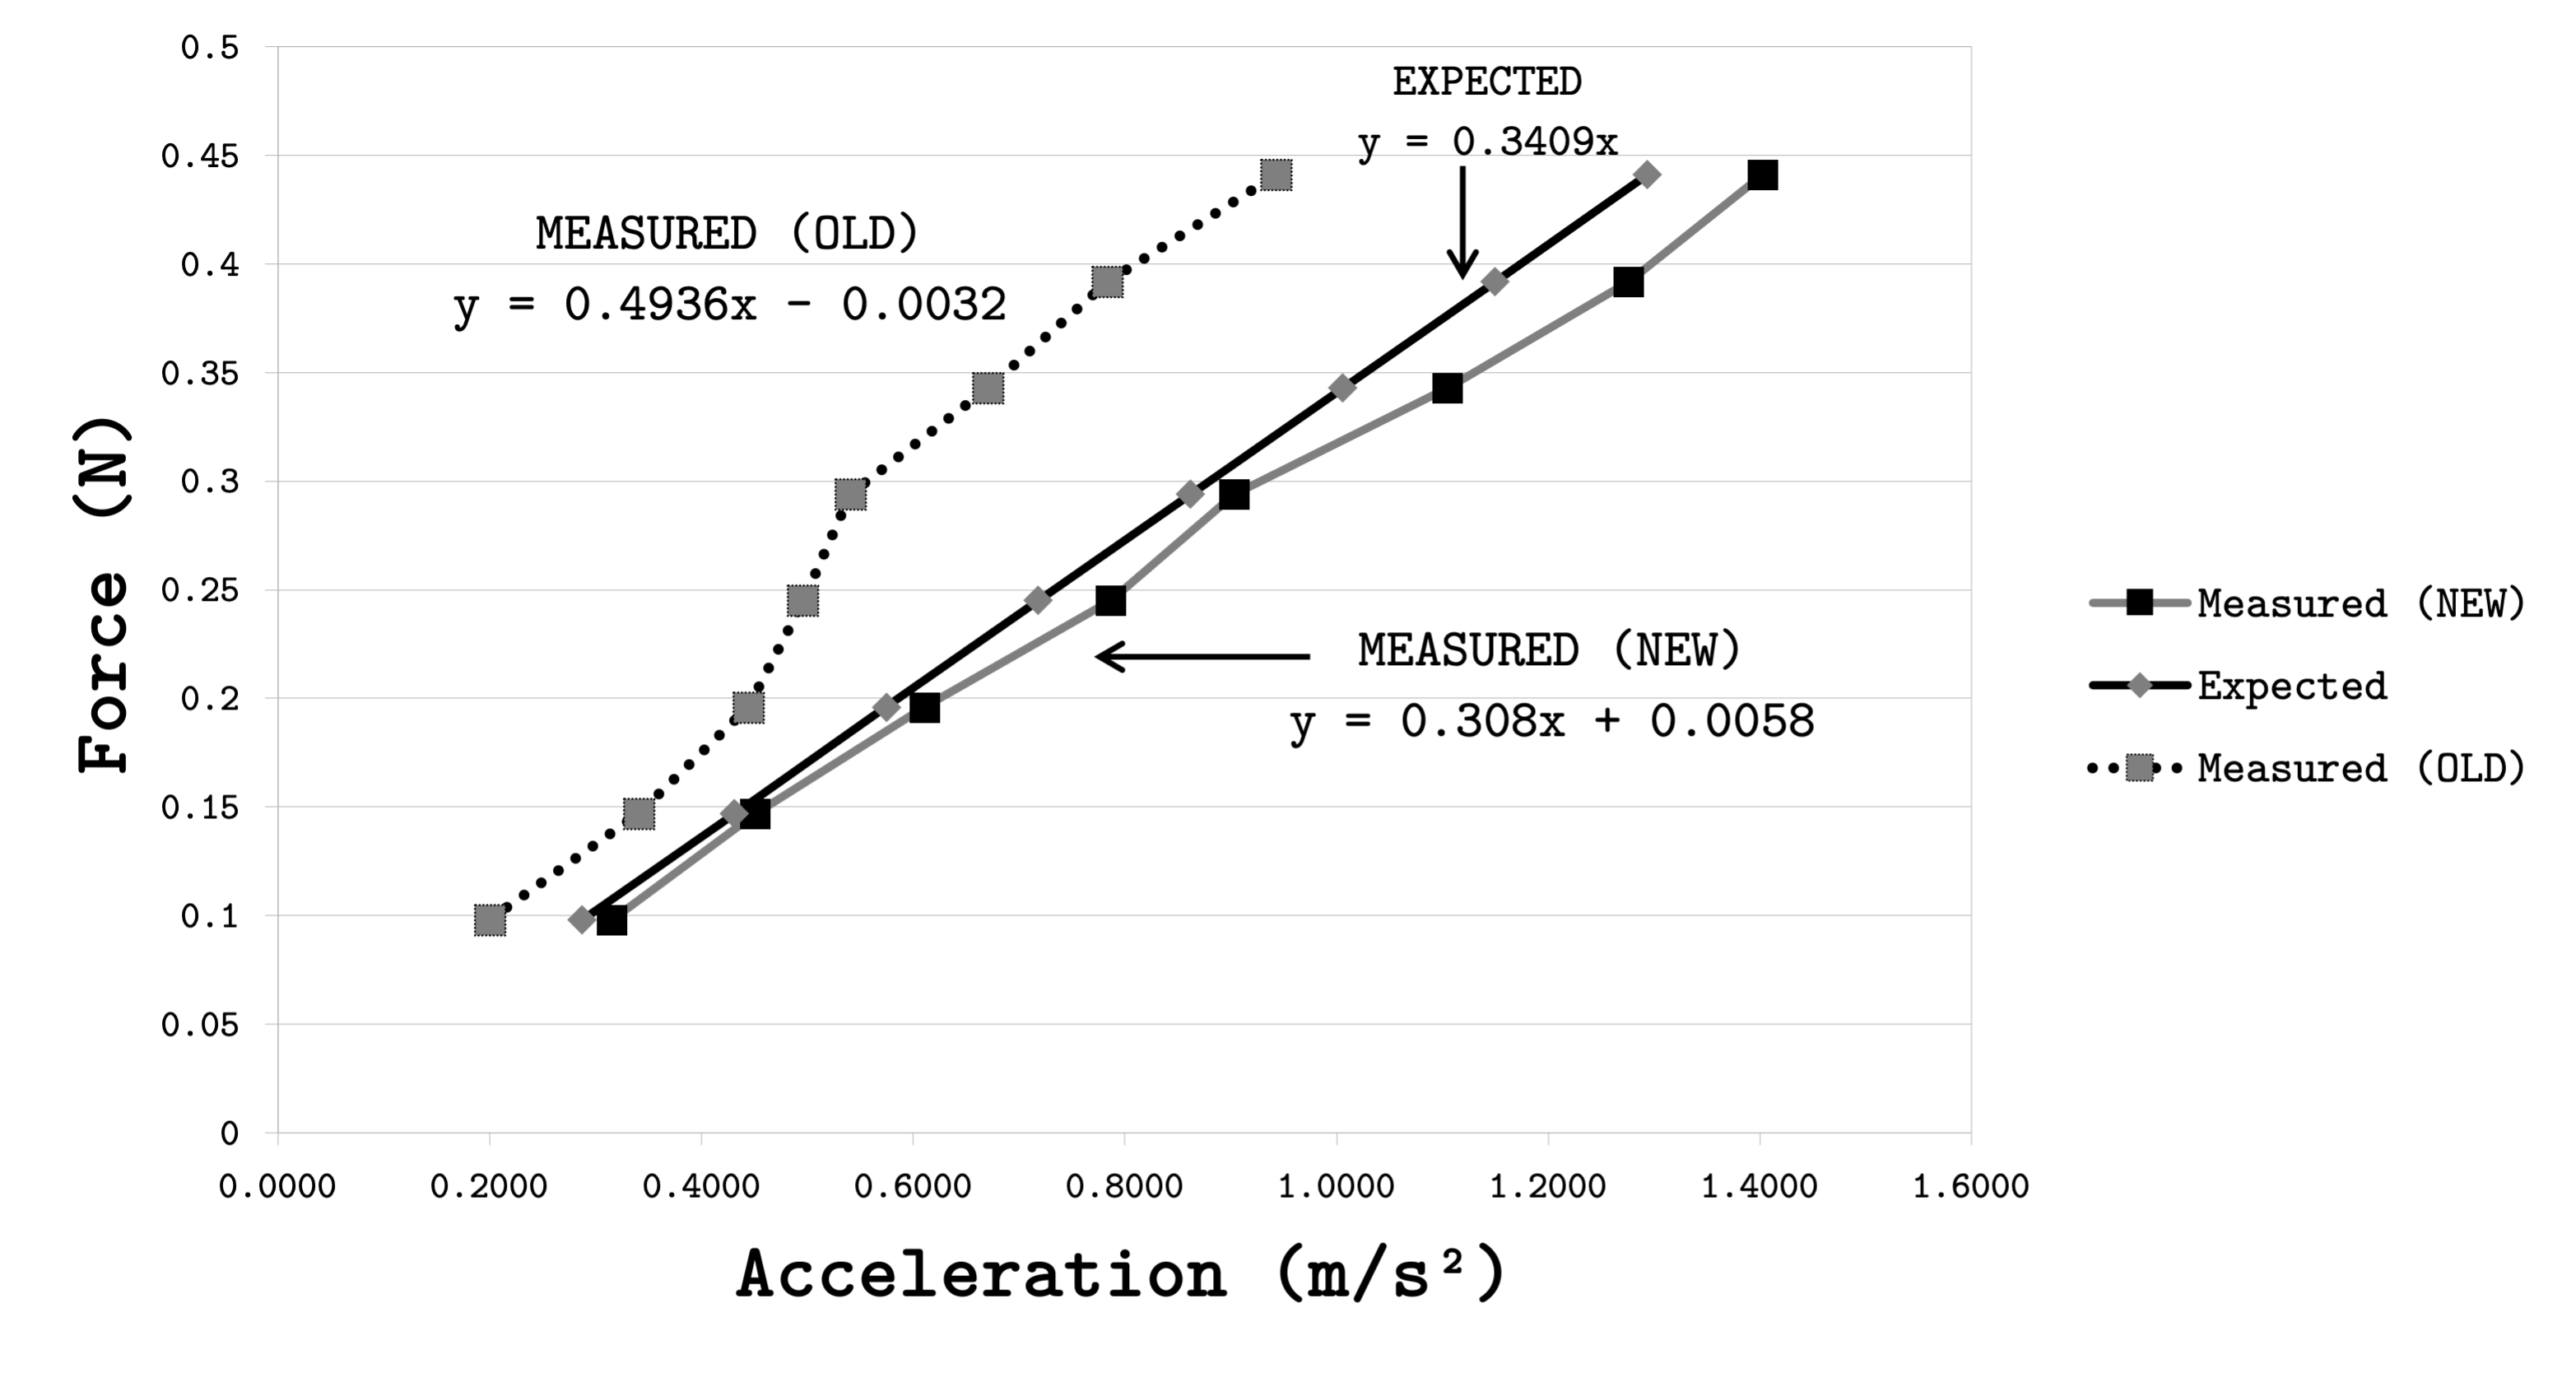
\includegraphics[width=0.90\columnwidth]{images/GraphFvA}
	\end{center}
\end{figure}
\end{landscape}

%----GRAPHS-----%

\newpage

